%% It is just an empty TeX file.
%% Write your code here.
\subsection{Casos simulados - II Enfermería}
Los siguientes casos descritos fueron pensados en su totalidad por María Fuencisla Sanz para el curso 2022/2023, en el contexto de las simulaciones y seminarios para la asignatura de Prácticas Clínicas (II Grado en Enfermería). El concepto general que subyace a todos ellos es, por una parte, evaluar las competencias técnicas (correcta toma de signos vitales (dolor, tensión arterial, saturación, frecuencias respiratoria y cardiaca, temperatura y glucemia (si el caso indicaba diabetes)), correcta higiene del paciente encamado, correcta administración de medicamentos), y por otro, desarrollar una serie de habilidades como el pensamiento crítico, comunicación interpersonal y evaluación de la gestión al estrés y consejos en el plano de la comunicación con el entorno del paciente.

Se diferencian dos tipos de casos, ambos se evaluarán con la rúbrica contenida en la tabla \ref{tab:PlanXVII:RubricaUCM}: el caso de higiene/Simulación del paciente encamado, que es una higiene normal, hecha por dos alumnas y que como único elemento a tener en cuenta es si el paciente es o no continente, decisión que se tomará en el momento. Los casos de simulación propiamente dichos (ver esquema en la figura \ref{fig:PlanXVII:FlujogramaGeneral}), desarrollados individualmente, tienen un componente de <<gestión de eventos emergentes/urgentes>>, esto es, hay un suceso interruptor en el que el alumnado tendrá que decidir si lo soluciona, bien movilizando al paciente por dolor, bien dándole algún tipo de medicamento o remedio o bien avisando en caso de que no pueda gestionarlo por si mismos. 

\begin{figure}[H]
    \centering
	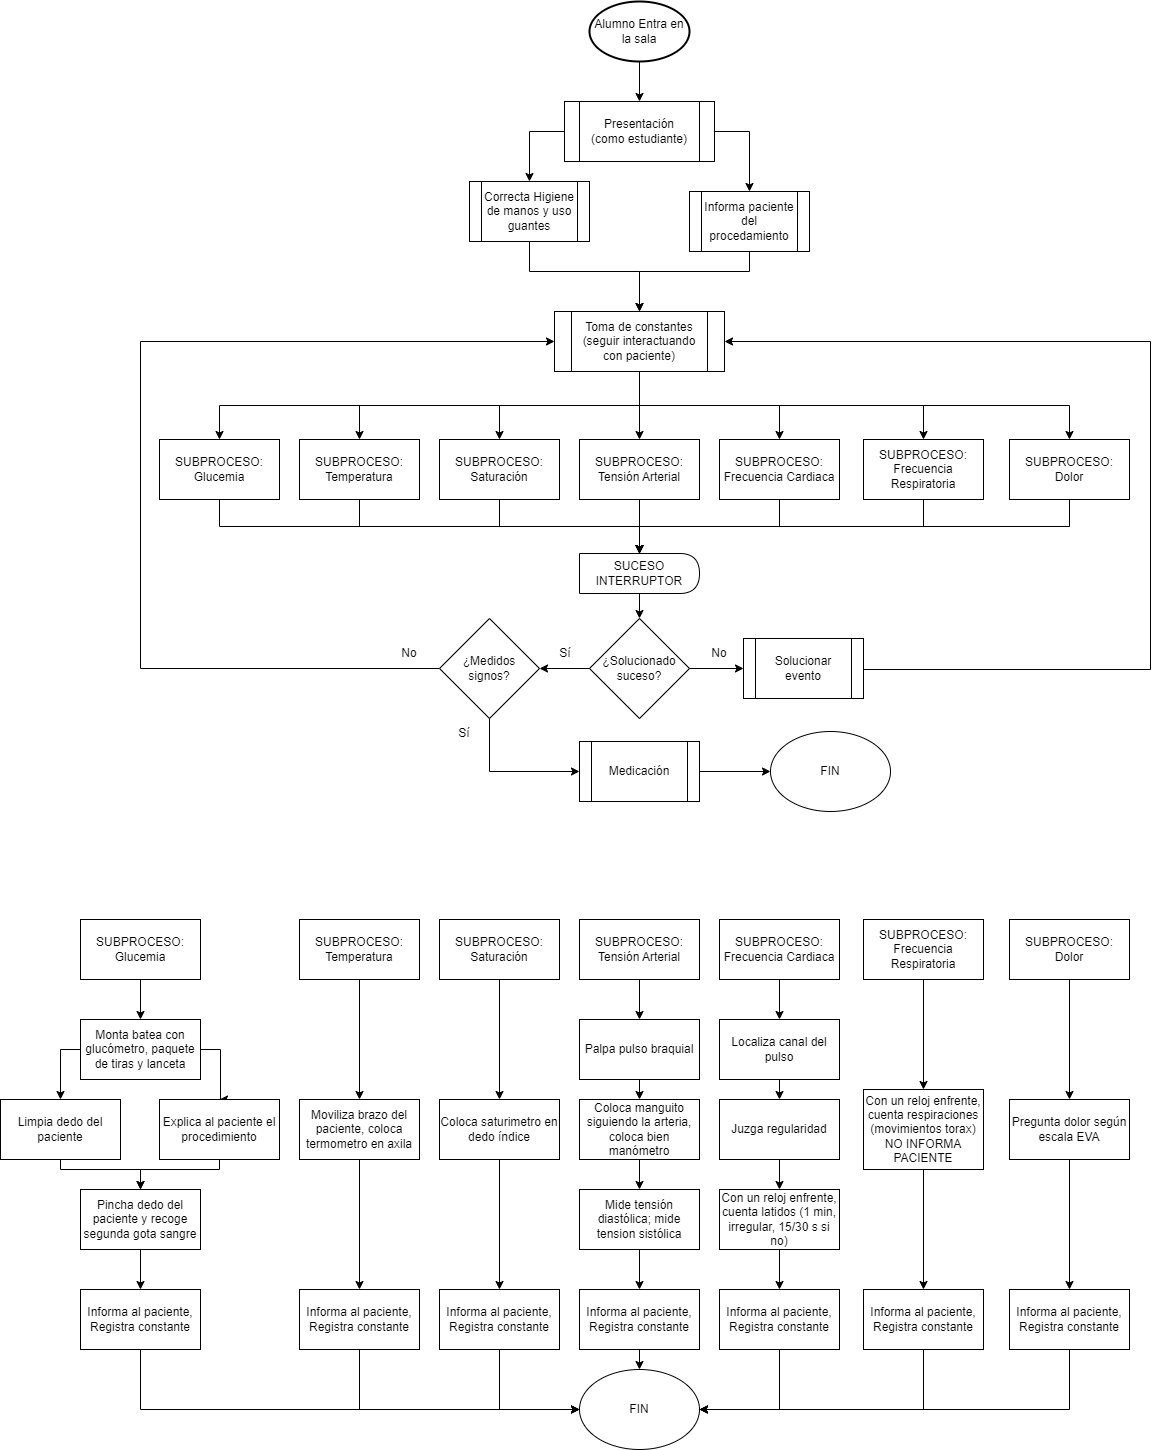
\includegraphics[width=0.8\textwidth]{./imagenes/ACV-AdSC-ResolucionGeneralCasosIIEnf.png}
	\caption{\label{fig:PlanXVII:FlujogramaGeneral}Flujograma general de los casos.}
\end{figure}
\clearpage
\subsubsection{Caso I - Dolor precordial Sancha}
    \begin{multicols}{2}
        \paragraph{Información general}
        \subparagraph{Escenario}: Planta
        \subparagraph{Paciente}: Mujer de 50 años ingresa con diagnostico medico de Fibrilación auricular. No hipertensa, diabética, alergia a amoxicilina. Tratamiento con insulina (10 U de Humalog, 5 U de Novorapid).
        \begin{itemize}[topsep=0pt, partopsep=0pt,itemsep=0pt,parsep=0pt]
            \item TA: 130/80 mmHg.
            \item FC: 102 Arrítmica (Fibrilación auricular).
            \item FR: 16 rpm
            \item Saturación: 98\%
            \item Dolor: 0
            \item Temperatura: 37 C
            \item Glucemia: 82 mg/dL
        \end{itemize}
        \subparagraph{Caso}: Se le da el parte al alumnado. Una vez iniciada la toma de constantes, referir un dolor en el pecho muy fuerte. Lo que se busca es que pida ayuda (por su nivel de formación, no puede hacer otra cosa) antes de seguir tomando constantes, insistiendo en el dolor si no lo hace. Si pide ayuda, responder como que ahora traen el electrocardiógrafo. Continuar con la toma de constantes y con la medicación
        \columnbreak
        \paragraph{Información para el alumno (Parte)}
        \subparagraph{} Sancha es una mujer de 50 años que está en estudio por una fribilación auricular. No es hipertensa pero sí diabética y es alérgica a la amoxicilina. Es algo quejosa y no le gustan nada los pinchazos. Tiene como Tratamiento unicamente insulina: humalog (15 U) y novorapid (5 U)
    \end{multicols}
    \begin{figure}[H]
        \centering
    	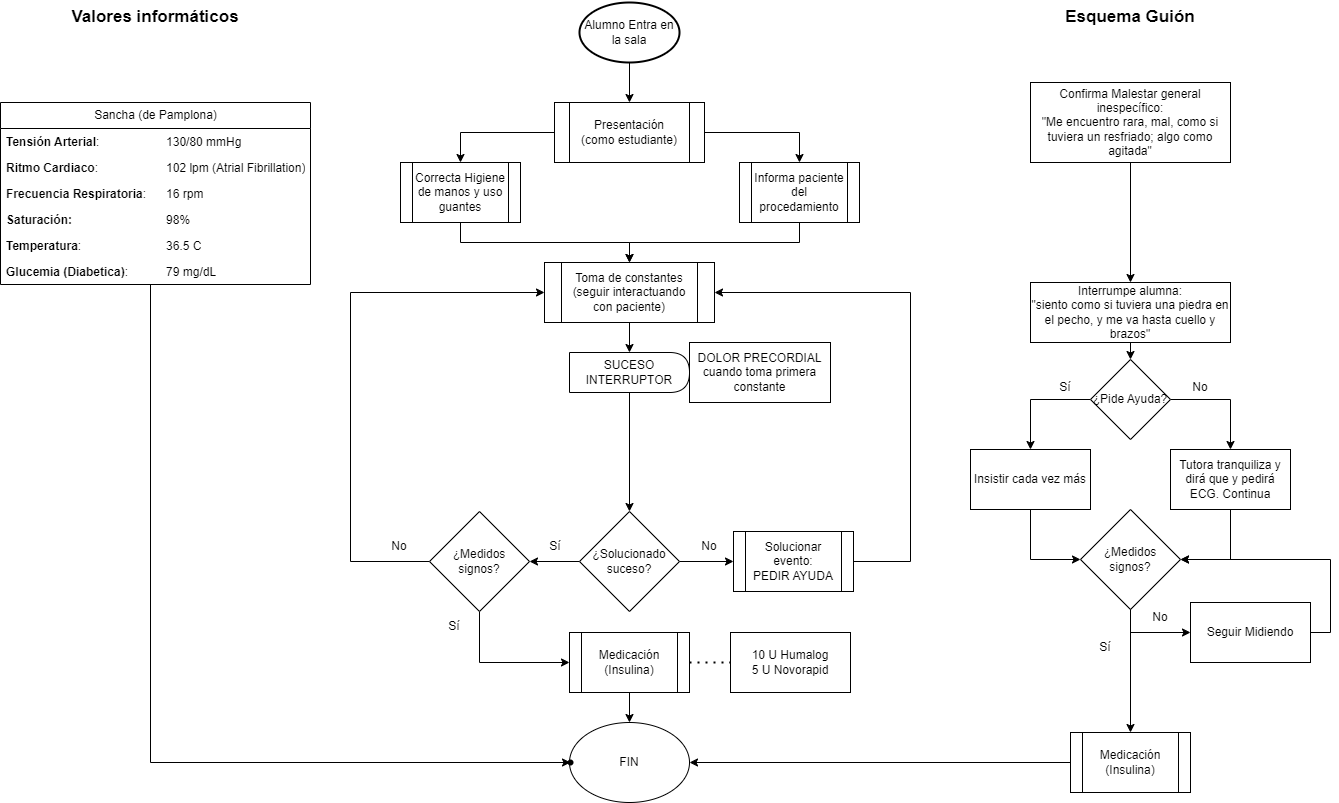
\includegraphics[width=\textwidth]{./imagenes/ACV-AdSC-CasoIDiagramaFlujoIIEnf.png}
    	\caption{\label{fig:PlanXVII:CasoI}Flujograma del Caso I.}
    \end{figure}
\clearpage
\subsubsection{Caso II - Hipotensión en Hipertensa Urraca}
\begin{multicols}{2}
    \paragraph{Información general}
    \subparagraph{Escenario}: Planta
    \subparagraph{Paciente}: Mujer de 60 años ingresa con diagnóstico médico de dolor abdominal sin filiar. Hipertensa, diabética. Tratamiento con insulina (7 U de Humalog, 4 U de Novorapid).
    \begin{itemize}[topsep=0pt, partopsep=0pt,itemsep=0pt,parsep=0pt]
        \item TA: 90/50 mmHg
        \item FC: 120 Sinusal
        \item FR: 16 rpm
        \item Saturación: 97 \%
        \item Dolor: 0
        \item Temperatura: 36,8 C
        \item Glucemia: 82 mg/dL
    \end{itemize}
    \subparagraph{Caso}: Se le da el parte al alumnado. Al entrar, la paciente se queja de debilidad. Se busca que el alumnado se fije en la hipotensión y que la integre con lo que se la ha dicho (que es hipertensa) y pida ayuda. Continuar con la toma de constantes y con la medicación.
    \columnbreak
    \paragraph{Información para el alumno (Parte)}
    \subparagraph{} Urraca es una mujer de 60 años ingresa con diagnóstico médico de dolor abdominal sin filiar. Hipertensa, diabética (insulina humalog 7 U, Novorapid 4 U). Se le ha retirado toda la medicación salvo la insulina.
\end{multicols}
\begin{figure}[H]
    \centering
	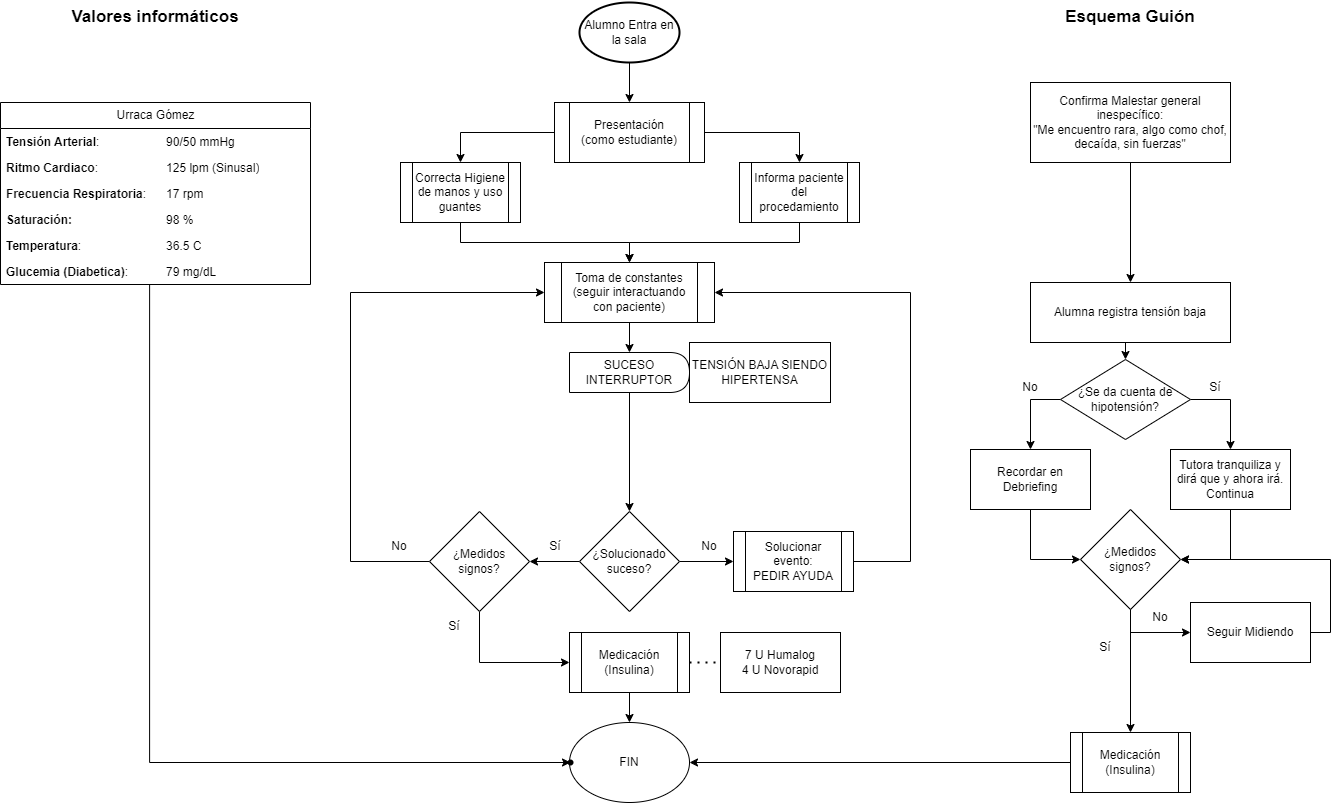
\includegraphics[width=\textwidth]{./imagenes/ACV-AdSC-CasoIIDiagramaFlujoIIEnf.png}
	\caption{\label{fig:PlanXVII:CasoII}Flujograma del Caso II.}
\end{figure}
\clearpage
\subsubsection{Caso III - Fiebre Inés}
\begin{multicols}{2}
    \paragraph{Información general}
    \subparagraph{Escenario}: Planta
    \subparagraph{Paciente}: Mujer de de 75 años ingresa con diagnóstico médico de EPOC agudizada Hipertensión arterial, no diabetes en tratamiento con inhaladores (plumicor) y reposo absoluto.
    \begin{itemize}[topsep=0pt, partopsep=0pt,itemsep=0pt,parsep=0pt]
        \item TA: 130/80 mmHg
        \item FC: 80 Sinusal
        \item FR: 12 rpm
        \item Saturación: 87 \%
        \item Dolor: 0
        \item Temperatura: 38,8 C
    \end{itemize}
    \subparagraph{Caso}: Nada más entrar, decir que tiene ganas de hacer pis (comprobar que tenga pañal) y pedir la cuña. Se busca que traigan la cuña y no le pidan que miccione en el pañal. Al continuar, relatar malestar general y algo de frío, confirmando las sospechas con toma te temperatura. Continuar con la toma de constantes y con la medicación.
    \columnbreak
    \paragraph{Información para el alumno (Parte)}
    \subparagraph{} Inés es una mujer de 75 años, con EPOC, que ha sido ingresada por una agudización de la EPOC. Tiene tratamiento con inhaladores (plumicor) y le han recomendando reposo absoluto, por lo que no puede ir al baño sola.
\end{multicols}
\begin{figure}[H]
    \centering
	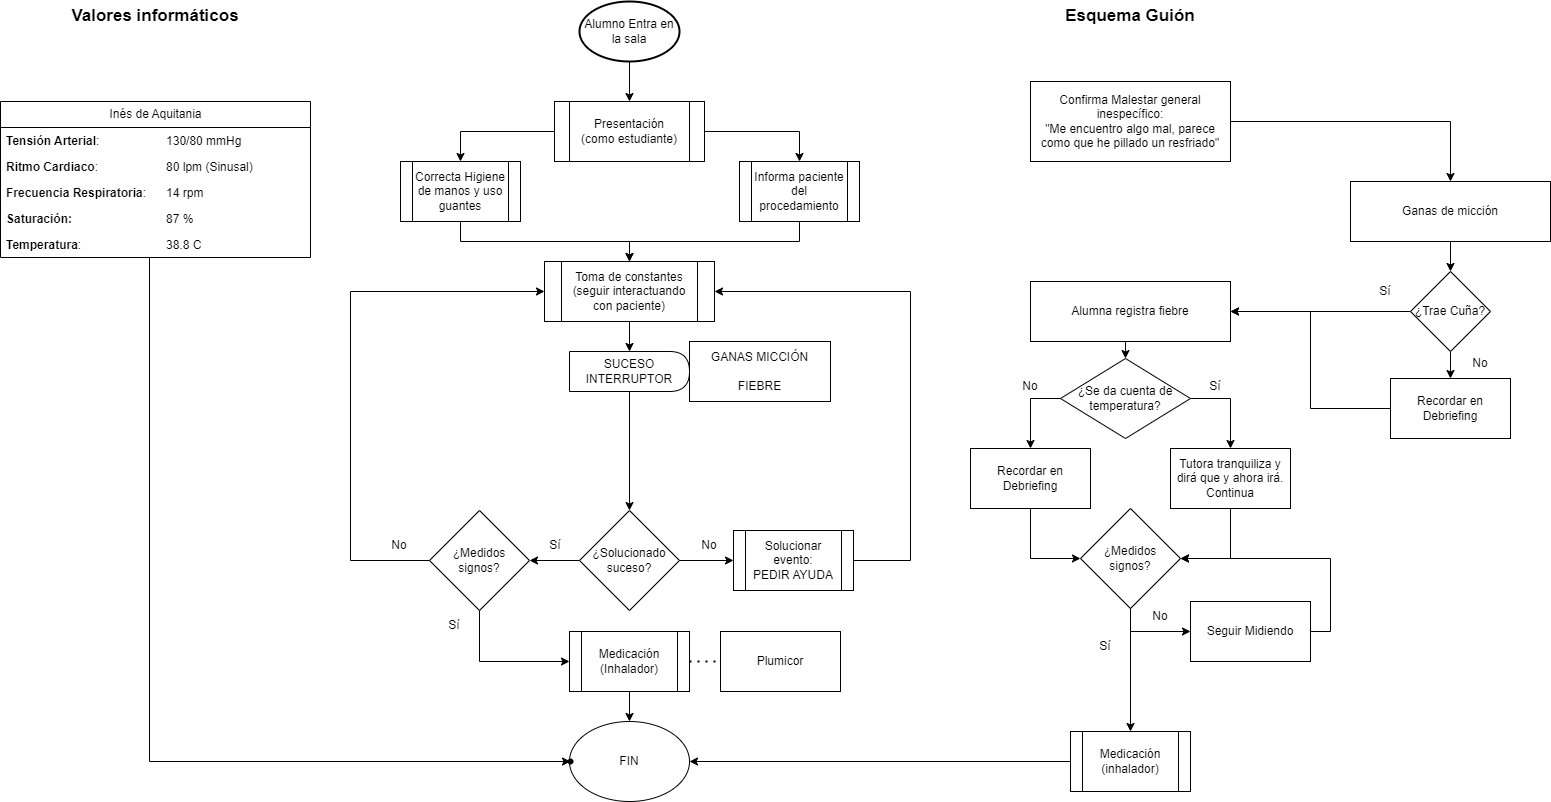
\includegraphics[width=\textwidth]{./imagenes/ACV-AdSC-CasoIIIDiagramaFlujoIIEnf.png}
	\caption{\label{fig:PlanXVII:CasoIII}Flujograma del Caso III.}
\end{figure}
\clearpage
\subsubsection{Caso IV - Dolor Constanza}
\begin{multicols}{2}
    \paragraph{Información general}
    \subparagraph{Escenario}: Planta
    \subparagraph{Paciente}: Mujer de 40 años ingresa con diagnóstico médico de accidente cerebro-vascular. No hipertensión arterial, no diabetes. Presenta disfagia a líquidos. Su tratamiento es AINEs (dolicatil) si dolor.
    \begin{itemize}[topsep=0pt, partopsep=0pt,itemsep=0pt,parsep=0pt]
        \item TA: 120/80 mmHg
        \item FC: 88 Sinusal
        \item FR: 16 rpm
        \item Saturación: 97 \%
        \item Dolor: EVA 8, espalda, incomodidad
        \item Temperatura: 37 C
    \end{itemize}
    \subparagraph{Caso}: Nada más entrar, decir que tiene mucho dolor en la espalda. Se busca que la alumna movilice al paciente y pase la escala EVA. Continuar con la toma de constantes y con la medicación.
    \columnbreak
    \paragraph{Información para el alumno (Parte)}
    \subparagraph{} Constanza es una mujer de 40 años que está recuperandose de un accidente cerebro-vascular. No tiene otras complicaciones (ni hipertensión ni diabetes) salvo disfagia a líquidos. Dado que lleva algo de tiempo en cama, el médico ha prescrito dolicatil si tiene dolor.
\end{multicols}
\begin{figure}[H]
    \centering
	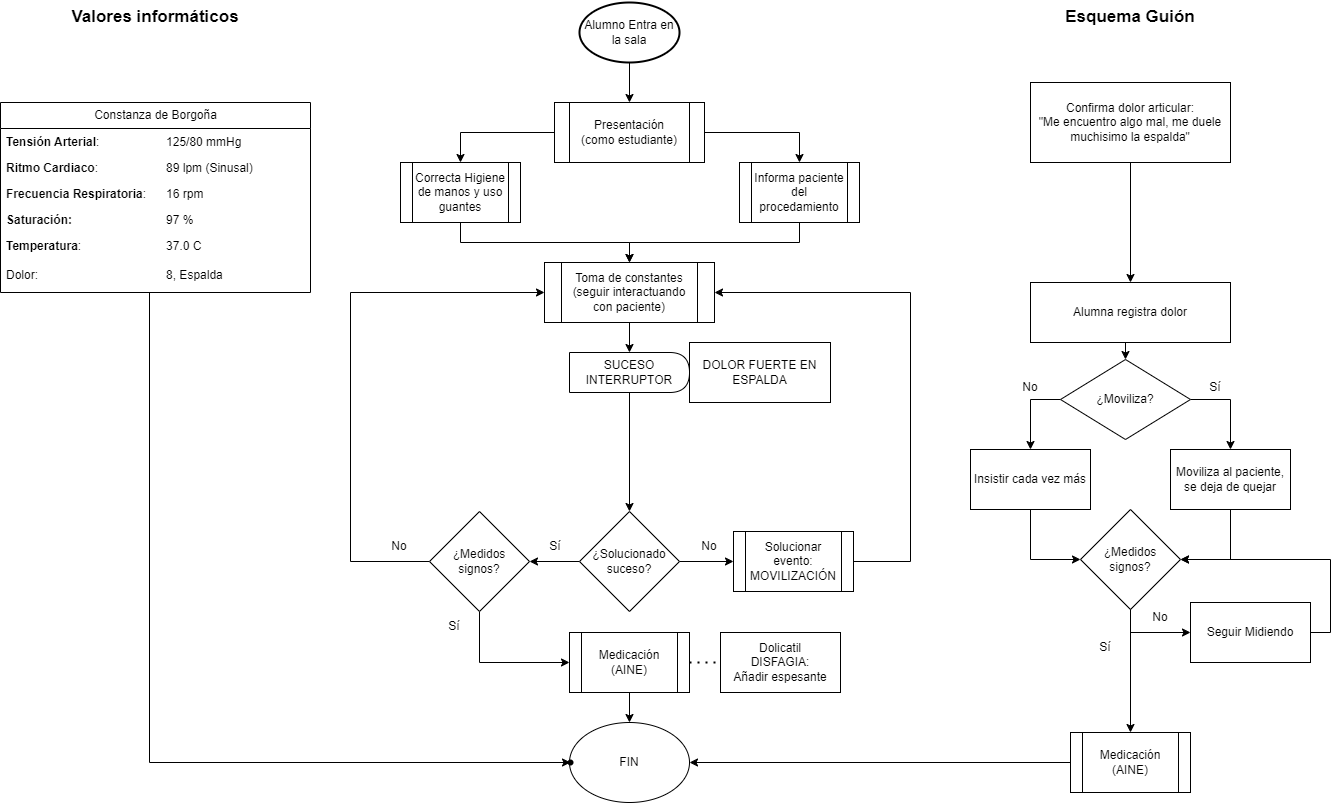
\includegraphics[width=\textwidth]{./imagenes/ACV-AdSC-CasoIVDiagramaFlujoIIEnf.png}
	\caption{\label{fig:PlanXVII:CasoIV}Flujograma del Caso IV.}
\end{figure}
\clearpage
\subsubsection{Caso V - Hipoglucemia Berta}
\begin{multicols}{2}
    \paragraph{Información general}
    \subparagraph{Escenario}: Planta
    \subparagraph{Paciente}: Mujer de 80 años ingresa con diagnóstico médico de fractura de cadera, teniendo de antecedentes: Hipertensión arterial, diabetes, Hipercolesterolemia. Tiene como tratamiento insulina y adalat retard 60 mg.
    \begin{itemize}[topsep=0pt, partopsep=0pt,itemsep=0pt,parsep=0pt]
        \item TA: 150/90 mmHg
        \item FC: 84 Sinusal
        \item FR: 18 rpm
        \item Saturación: 97 \%
        \item Dolor: EVA 4, cadera, incomodidad
        \item Temperatura: 36,8
        \item Glucemia: 50 mg/dL
    \end{itemize}
    \subparagraph{Caso}: Al entrar en la habitación nos dice que se encuentra mal, mareada, con sudoración fría (sospechas de hipoglucemia severa). Se busca que la alumna reaccione rápidamente dando algo con azúcar para tratar de revertirlo. Continuar con la toma de constantes y con la medicación.
    \columnbreak
    \paragraph{Información para el alumno (Parte)}
    \subparagraph{} Berta es una mujer de 80 años que está en planta recuperandose de una operación de cadera. Es hipertensa (tiene como medicación adalat retard 60 mg), con problemas de colesterol (sin tratamiento de momento) y diabética (ozempic). Se ha levantado con algo de nauseas y no ha desayunado.
\end{multicols}
\begin{figure}[H]
    \centering
	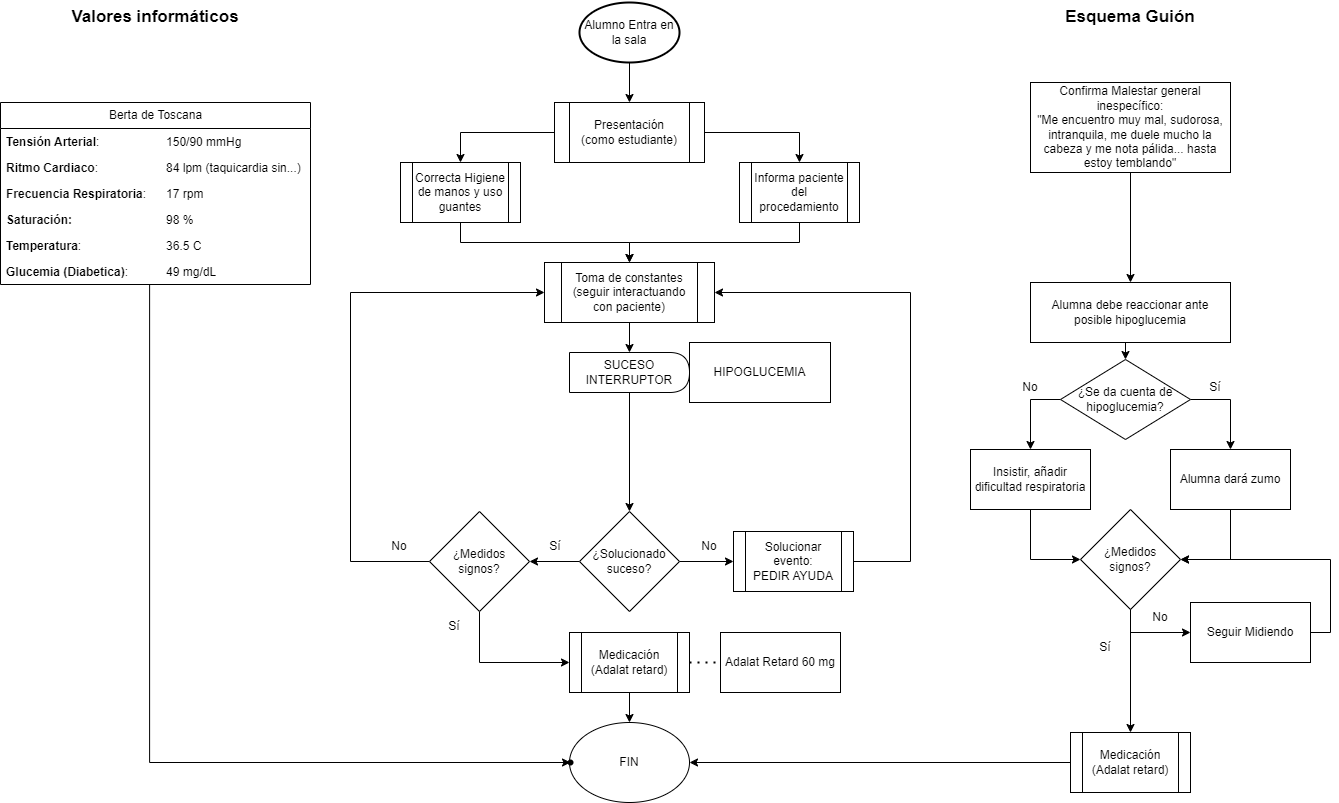
\includegraphics[width=\textwidth]{./imagenes/ACV-AdSC-CasoVDiagramaFlujoIIEnf.png}
	\caption{\label{fig:PlanXVII:CasoV}Flujograma del Caso V.}
\end{figure}



